\section*{Procedimentos}
% Estilos dos diagramas (etapa, io, seta, ...) definidos em config/preambulo.tex.

\subsection*{Método dos perfis delgados}

A teoria dos perfis delgados~\cite{anderson} admite escoamento potencial e
incompressível, e perfil com espessura, curvatura e ângulo de ataque pequenos.
O perfil é substituído pela sua linha média, sobre a qual se distribui uma folha
de vórtices de intensidade $\gamma$. Impondo que a linha média seja uma linha de
corrente e a condição de Kutta no bordo de fuga, $\gamma(\pi) = 0$, obtém-se,
com a mudança de variável $x = \tfrac{c}{2}(1-\cos\theta)$, a solução em série
de Fourier
\[
  \gamma(\theta) = 2V_\infty\left[A_0\,\frac{1+\cos\theta}{\sin\theta}
  + \sum_{n=1}^{\infty} A_n \sin n\theta\right],
\]
cujos coeficientes dependem apenas do declive da linha média, $dz_c/dx$. Para o
coeficiente de sustentação bastam os dois primeiros, $A_0$ e $A_1$; o perfil é
então representado só pela linha média, e a espessura e a viscosidade são
ignoradas.

A aplicação do método, implementada em MATLAB, está esquematizada na
Figura~\ref{fig:diag_thin}, com as entradas de cada etapa à esquerda e as saídas
à direita.

\begin{figure}[H]
\centering
\begin{tikzpicture}[node distance=0.45cm]
  % etapas
  \node[etapa] (e1) {\textbf{1.} Importação da geometria};
  \node[etapa, below=of e1] (e2) {\textbf{2.} Interpolação e linha média};
  \node[etapa, below=of e2] (e3) {\textbf{3.} Declive e mudança de variável $x \rightarrow \theta$};
  \node[etapa, below=of e3] (e4) {\textbf{4.} Coeficientes de Fourier};
  \node[etapa, below=of e4] (e5) {\textbf{5.} Coeficientes aerodinâmicos};
  \node[etapa, below=of e5] (e6) {\textbf{6.} Estudo de convergência em $N$};
  \foreach \a/\b in {e1/e2,e2/e3,e3/e4,e4/e5,e5/e6}
    \draw[seta] (\a) -- (\b);
  % entradas
  \node[io, left=0.5cm of e1, align=flush right] (i1) {Ficheiro de coordenadas (formato Lednicer): 36 pontos no extradorso e 36 no intradorso};
  \node[io, left=0.5cm of e2, align=flush right] (i2) {$(x_u,z_u)$, $(x_l,z_l)$; $N = 1000$ pontos};
  \node[io, left=0.5cm of e3, align=flush right] (i3) {$z_c(x)$; $x = \tfrac{1}{2}(1-\cos\theta)$};
  \node[io, left=0.5cm of e4, align=flush right] (i4) {$dz_c/dx\,(\theta)$, $\theta \in [0,\pi]$};
  \node[io, left=0.5cm of e5, align=flush right] (i5) {$I_0$, $A_1$; $\alpha \in [-20^\circ, 20^\circ]$, passo $0{,}5^\circ$};
  \node[io, left=0.5cm of e6, align=flush right] (i6) {8 valores de $N$ entre 50 e $10\,000$ (referência: $N = 10\,000$); tolerâncias $\Delta c_l = 10^{-3}$, $\Delta\alpha_{L=0} = 0{,}01^\circ$};
  % saídas
  \node[io, right=0.5cm of e1] (o1) {$(x_u,z_u)$, $(x_l,z_l)$, normalizados pela corda};
  \node[io, right=0.5cm of e2] (o2) {$z_c(x) = \tfrac{1}{2}(z_u+z_l)$};
  \node[io, right=0.5cm of e3] (o3) {$dz_c/dx\,(\theta)$};
  \node[io, right=0.5cm of e4] (o4) {$I_0$, $A_1$ (regra dos trapézios)};
  \node[io, right=0.5cm of e5] (o5) {$\alpha_{L=0}$, $c_l(\alpha)$, $dc_l/d\alpha = 2\pi$};
  \node[io, right=0.5cm of e6] (o6) {Erros de $c_l(5^\circ)$ e $\alpha_{L=0}$ em função de $N$; verificação de que $N = 1000$ cumpre as tolerâncias};
  \foreach \k in {1,...,6} {
    \draw[setaio] (i\k) -- (e\k);
    \draw[setaio] (e\k) -- (o\k);
  }
  \path (e1.north) ++(0,0.6) coordinate (topo);
  \node[titulo] at (i1 |- topo) {Entradas};
  \node[titulo] at (o1 |- topo) {Saídas};
\end{tikzpicture}
\caption{Diagrama de blocos do método dos perfis delgados.}
\label{fig:diag_thin}
\end{figure}

\begin{etapas}
  \item \textbf{Importação da geometria.} Usaram-se as coordenadas da base de
  dados da UIUC (formato Lednicer), com 36 pontos por superfície, já
  normalizadas pela corda.
  \item \textbf{Interpolação e linha média.} Como o ficheiro não dá a linha
  média, e o extradorso e o intradorso não estão definidos nos mesmos $x$,
  interpolaram-se as duas superfícies nos mesmos $N$ pontos e calculou-se a
  linha média como a média das duas~\cite{abbott}:
  \[
    z_c(x) = \frac{z_u(x) + z_l(x)}{2}.
  \]
  Usou-se interpolação \emph{pchip} em função de $\sqrt{x}$: a variável
  $\sqrt{x}$ espaça os pontos junto ao bordo de ataque, onde a curvatura é
  maior, e a \emph{pchip} não cria as oscilações de um polinómio de grau
  elevado entre pontos. A Figura~\ref{fig:geom} mostra o perfil e a linha média
  obtida.
\end{etapas}

\begin{figure}[H]
  \centering
  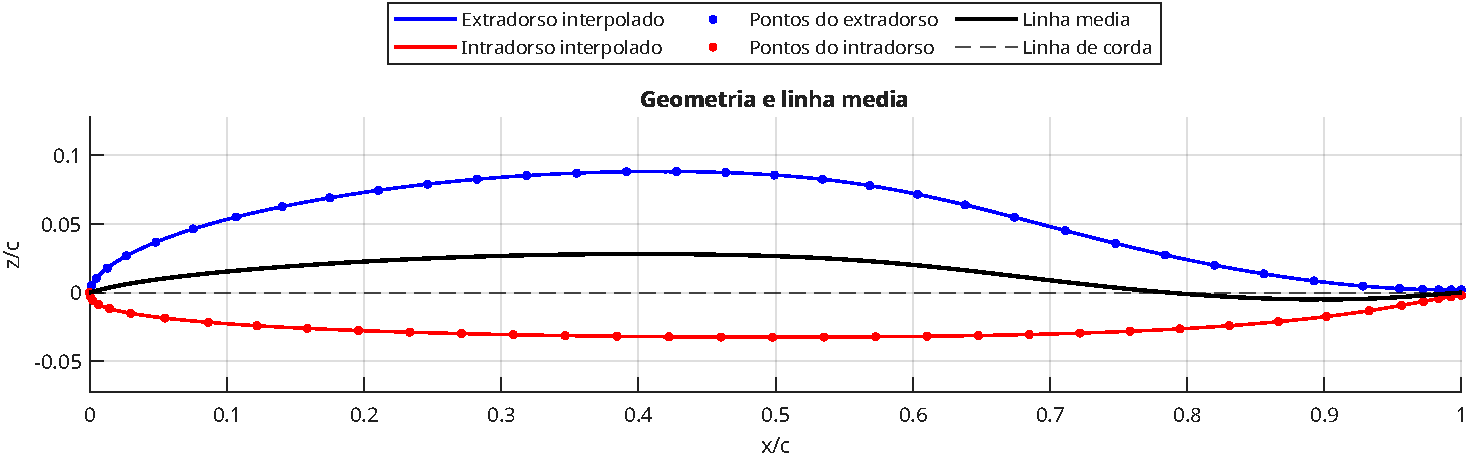
\includegraphics[width=0.7\textwidth]{imagens/geometry.pdf}
  \caption{Perfil Roncz/Marske-7 e respetiva linha média.}
  \label{fig:geom}
\end{figure}

\begin{etapas}[resume]
  \item \textbf{Declive e mudança de variável.} O declive $dz_c/dx$ foi
  calculado por diferenças finitas centradas e reinterpolado numa malha
  uniforme em $\theta$, através de
  \[
    x = \frac{c}{2}\,(1 - \cos\theta), \qquad 0 \le \theta \le \pi ,
  \]
  em que $\theta = 0$ é o bordo de ataque e $\theta = \pi$ o bordo de fuga. Uma
  malha uniforme em $\theta$ concentra os pontos junto aos dois bordos.
  \item \textbf{Coeficientes de Fourier.} Os integrais foram calculados pela
  regra dos trapézios:
  \[
    A_0 = \alpha - I_0, \qquad
    I_0 = \frac{1}{\pi}\int_0^{\pi} \frac{dz_c}{dx}\,d\theta, \qquad
    A_1 = \frac{2}{\pi}\int_0^{\pi} \frac{dz_c}{dx}\cos\theta\,d\theta .
  \]
  $I_0$ e $A_1$ dependem só da geometria, pelo que se calculam uma única vez;
  só $A_0$ varia com $\alpha$.
  \item \textbf{Coeficientes aerodinâmicos.} Para $\alpha$ entre $-20^\circ$ e
  $20^\circ$, com passo de $0{,}5^\circ$, o coeficiente de sustentação é
  \[
    c_l = 2\pi\left(A_0 + \frac{A_1}{2}\right) = 2\pi\,(\alpha - \alpha_{L=0}),
    \qquad \alpha_{L=0} = I_0 - \frac{A_1}{2}.
  \]
  O declive é $dc_l/d\alpha = 2\pi$~rad$^{-1}$ para qualquer perfil, e a
  curvatura entra apenas no ângulo de sustentação nula, $\alpha_{L=0}$.
  \item \textbf{Convergência.} Repete-se o cálculo para oito valores de $N$
  entre 50 e $10\,000$ e comparam-se $c_l(5^\circ)$ e $\alpha_{L=0}$ com os valores para
  $N = 10\,000$. As tolerâncias ($10^{-3}$ e $0{,}01^\circ$) são cumpridas a
  partir de $N = 200$; com o valor usado, $N = 1000$, os erros são
  $7{,}2\times10^{-5}$ e $6{,}6\times10^{-4}$\,$^\circ$. Como o custo é desprezável
  ($\approx 0{,}1$~ms por cálculo), usou-se $N = 1000$ como margem de segurança.
\end{etapas}


\subsection*{Método dos painéis}

Utilizou-se o método dos painéis de vórtices com intensidade linear
\cite{katz}, implementado em MATLAB e esquematizado na
Figura~\ref{fig:diag_paineis}.

\begin{figure}[H]
\centering
\begin{tikzpicture}[node distance=0.45cm]
  \node[etapa] (p1) {\textbf{1.} Painelização do perfil};
  \node[etapa, below=of p1] (p2) {\textbf{2.} Coeficientes de influência};
  \node[etapa, below=of p2] (p3) {\textbf{3.} Condições de fronteira};
  \node[etapa, below=of p3] (p4) {\textbf{4.} Resolução do sistema linear};
  \node[etapa, below=of p4] (p5) {\textbf{5.} Velocidade tangencial e $C_p$};
  \node[etapa, below=of p5] (p6) {\textbf{6.} Coeficientes de força};
  \node[etapa, below=of p6] (p7) {\textbf{7.} Pós-processamento};
  \foreach \a/\b in {p1/p2,p2/p3,p3/p4,p4/p5,p5/p6,p6/p7}
    \draw[seta] (\a) -- (\b);
  % ciclo de convergência
  \draw[seta, dashed] (p6.east) -- ++(0.3,0) |- (p1.east);
  % entradas
  \node[io, left=0.5cm of p1, align=flush right] (j1) {Ficheiro de coordenadas; número de painéis $N$};
  \node[io, left=0.5cm of p2, align=flush right] (j2) {Nós $(x_j,z_j)$; pontos de controlo $(x_i,z_i)$};
  \node[io, left=0.5cm of p3, align=flush right] (j3) {$V_\infty$, $\alpha$; normais $\mathbf{n}_i$};
  \node[io, left=0.5cm of p4, align=flush right] (j4) {Matriz $\mathbf{A}$, vetor $\mathbf{b}$};
  \node[io, left=0.5cm of p5, align=flush right] (j5) {$\gamma_j$; influências; tangentes $\mathbf{t}_i$};
  \node[io, left=0.5cm of p6, align=flush right] (j6) {$C_{p,i}$, $\mathbf{n}_i$, $\Delta s_i$, $\alpha$};
  \node[io, left=0.5cm of p7, align=flush right] (j7) {$\gamma_j$, $V_{t,i}$, $C_{p,i}$; malha de pontos em redor do perfil};
  % saídas
  \node[io, right=0.75cm of p1] (q1) {Nós, pontos de controlo, $\mathbf{t}_i$, $\mathbf{n}_i$, $\Delta s_i$};
  \node[io, right=0.75cm of p2] (q2) {Matriz $\mathbf{A}$, $(N{+}1)\times(N{+}1)$};
  \node[io, right=0.75cm of p3] (q3) {Vetor $\mathbf{b}$; condição de Kutta $\gamma_1 + \gamma_{N+1} = 0$};
  \node[io, right=0.75cm of p4] (q4) {Intensidades $\gamma_j$ nos $N+1$ nós};
  \node[io, right=0.75cm of p5] (q5) {$V_{t,i}$, $C_{p,i}$; verificação $V_{n,i} \approx 0$};
  \node[io, right=0.75cm of p6] (q6) {$C_x$, $C_z$ $\rightarrow$ $c_l$, $c_{d,p}$; $c_l(5^\circ)$ para $N = 20, 50, \dots, 800$ e erro relativo a $N = 800$};
  \node[io, right=0.75cm of p7] (q7) {Linhas de corrente, ponto de estagnação, $C_{p,\min}$};
  \foreach \k in {1,...,7} {
    \draw[setaio] (j\k) -- (p\k);
    \draw[setaio] (p\k) -- (q\k);
  }
  \path (p1.north) ++(0,0.6) coordinate (topo);
  \node[titulo] at (j1 |- topo) {Entradas};
  \node[titulo] at (q1 |- topo) {Saídas};
\end{tikzpicture}
\caption{Diagrama de blocos do método dos painéis. A seta a tracejado
representa o estudo de convergência em $N$.}
\label{fig:diag_paineis}
\end{figure}

\begin{etapas}
  \item \textbf{Painelização.} O contorno é percorrido no sentido anti-horário a
  partir do bordo de fuga; cada superfície é reinterpolada (\emph{pchip}) em
  $N/2$ painéis de igual comprimento de arco, com ponto de controlo no ponto
  médio, comprimento $\Delta s_i$, tangente $\mathbf{t}_i$ e normal exterior
  $\mathbf{n}_i$.
  \item \textbf{Coeficientes de influência.} A intensidade varia linearmente
  entre os valores nodais $\gamma_j$ e $\gamma_{j+1}$; a velocidade induzida
  calcula-se analiticamente no referencial local do painel, e $a_{ij}$ é a sua
  componente normal no ponto $i$ para $\gamma_j$ unitário.
  \item \textbf{Condições de fronteira.} Impermeabilidade nos pontos de
  controlo e condição de Kutta (aproximada, pois o bordo de fuga tem espessura
  finita):
  \[
    \sum_{j=1}^{N+1} a_{ij}\,\gamma_j = -\mathbf{V}_\infty \cdot \mathbf{n}_i ,
    \quad i = 1,\dots,N, \qquad \gamma_1 + \gamma_{N+1} = 0 .
  \]
  \item \textbf{Resolução.} O sistema $\mathbf{A}\boldsymbol{\gamma} = \mathbf{b}$
  resolve-se diretamente (operador \texttt{\textbackslash} do MATLAB).
  \item \textbf{Velocidade tangencial e $C_p$.} Somando $\mathbf{V}_\infty$ à
  velocidade induzida por todos os painéis,
  \[
    C_{p,i} = 1 - \left(\frac{V_{t,i}}{V_\infty}\right)^2 ,
  \]
  usando-se $V_{n,i} \approx 0$ para verificar a solução.
  \item \textbf{Coeficientes de força.} Integrando a pressão no contorno e
  projetando nas direções do escoamento livre,
  \[
    C_{x,z} = -\sum_i C_{p,i}\, n_{x,z,i}\,\Delta s_i , \qquad
    c_l = -C_x \sin\alpha + C_z \cos\alpha , \qquad
    c_{d,p} = C_x \cos\alpha + C_z \sin\alpha .
  \]
  Repete-se a $\alpha = 5^\circ$ para $N = 20, 50, \dots, 800$ (passo 30),
  comparando $c_l$ com o valor para $N = 800$ (seta a tracejado).
  \item \textbf{Pós-processamento.} Velocidade numa malha em redor do perfil
  (linhas de corrente), ponto de estagnação (mudança de sinal de $V_t$ junto ao
  bordo de ataque) e $C_{p,\min}$.
\end{etapas}


\subsection*{Simulação CFD}

A simulação foi realizada no OpenFOAM~\cite{openfoam}, segundo o procedimento da
Figura~\ref{fig:diag_cfd}.

\begin{figure}[H]
\centering
\begin{tikzpicture}[node distance=0.45cm]
  \node[etapa] (c1) {\textbf{1.} Geometria e domínio computacional};
  \node[etapa, below=of c1] (c2) {\textbf{2.} Geração da malha};
  \node[etapa, below=of c2] (c3) {\textbf{3.} Condições de fronteira e modelo físico};
  \node[etapa, below=of c3] (c4) {\textbf{4.} Resolução (\texttt{simpleFoam})};
  \node[etapa, below=of c4] (c5) {\textbf{5.} Coeficientes de força};
  \node[etapa, below=of c5] (c6) {\textbf{6.} Pós-processamento};
  \foreach \a/\b in {c1/c2,c2/c3,c3/c4,c4/c5,c5/c6}
    \draw[seta] (\a) -- (\b);
  % ciclo de convergência de malha
  \draw[seta, dashed] (c5.east) -- ++(0.3,0) |- (c2.east);
  % entradas
  \node[io, left=0.5cm of c1, align=flush right] (k1) {Coordenadas do perfil; dimensões do domínio [TODO]};
  \node[io, left=0.5cm of c2, align=flush right] (k2) {Domínio; número de células, $y^+$ pretendido, refinamento junto à parede [TODO]};
  \node[io, left=0.5cm of c3, align=flush right] (k3) {$V_\infty = 100$~m/s, $\nu = 10^{-5}$~m$^2$/s, $c = 1$~m, $\alpha$; modelo de turbulência e intensidade turbulenta [TODO]};
  \node[io, left=0.5cm of c4, align=flush right] (k4) {Caso configurado; esquemas numéricos; critério de paragem dos resíduos [TODO]};
  \node[io, left=0.5cm of c5, align=flush right] (k5) {Campos $p$ e $\mathbf{U}$; $c$, $V_\infty$; direções de sustentação e arrasto};
  \node[io, left=0.5cm of c6, align=flush right] (k6) {Campos convergidos para $\alpha = 0^\circ, 5^\circ, \dots, 20^\circ$};
  % saídas
  \node[io, right=0.75cm of c1] (r1) {Domínio 2D em torno do perfil};
  \node[io, right=0.75cm of c2] (r2) {Malha; qualidade (\texttt{checkMesh}) e $y^+$};
  \node[io, right=0.75cm of c3] (r3) {Caso pronto (\texttt{0/}, \texttt{constant/}, \texttt{system/})};
  \node[io, right=0.75cm of c4] (r4) {Campos $\mathbf{U}$, $p$ e turbulentos; histórico dos resíduos};
  \node[io, right=0.75cm of c5] (r5) {$c_l$, $c_d$ (\texttt{forceCoeffs}); ciclo de refinamento até $c_l$ deixar de variar};
  \node[io, right=0.75cm of c6] (r6) {Linhas de corrente, $C_p$ no perfil, ponto de estagnação, $C_{p,\min}$};
  \foreach \k in {1,...,6} {
    \draw[setaio] (k\k) -- (c\k);
    \draw[setaio] (c\k) -- (r\k);
  }
  \path (c1.north) ++(0,0.6) coordinate (topo);
  \node[titulo] at (k1 |- topo) {Entradas};
  \node[titulo] at (r1 |- topo) {Saídas};
\end{tikzpicture}
\caption{Diagrama de blocos da simulação CFD. A seta a tracejado representa o
estudo de convergência de malha.}
\label{fig:diag_cfd}
\end{figure}

\begin{etapas}
  \item \textbf{Geometria e domínio.} O perfil é importado a partir das
  coordenadas e envolvido por um domínio 2D de [TODO] cordas.
  \item \textbf{Malha.} Malha [TODO] com [TODO] células, refinada junto à parede
  para $y^+ \approx$~[TODO]; a qualidade verifica-se com \texttt{checkMesh}.
  \item \textbf{Condições de fronteira e modelo físico.} Velocidade uniforme
  $V_\infty$ na entrada, pressão fixa na saída e não escorregamento no perfil;
  $\alpha$ imposto [TODO: rodando $\mathbf{V}_\infty$ ou o perfil]. Resolvem-se as
  equações RANS 2D, estacionárias e incompressíveis, com o modelo de turbulência
  [TODO], com $Re = V_\infty c/\nu = 10^{7}$, próximo do valor em voo
  (Tabela~\ref{tab:sr22}):
  \[
    \nabla\cdot\overline{\mathbf{U}} = 0, \qquad
    (\overline{\mathbf{U}}\cdot\nabla)\,\overline{\mathbf{U}} =
    -\nabla \bar{p} + \nabla\cdot\left[(\nu + \nu_t)
    \left(\nabla\overline{\mathbf{U}} + \nabla\overline{\mathbf{U}}^{\mathsf{T}}\right)\right],
  \]
  onde $\bar{p}$ é a pressão cinemática (dividida por $\rho$).
  \item \textbf{Resolução.} Algoritmo SIMPLE (\texttt{simpleFoam}) até os
  resíduos descerem abaixo de [TODO] e $c_l$ estabilizar.
  \item \textbf{Coeficientes de força.} Integrando a pressão e as tensões
  viscosas no perfil (\texttt{forceCoeffs}),
  \[
    C_p = \frac{\bar{p} - \bar{p}_\infty}{\tfrac{1}{2}V_\infty^2}, \qquad
    c_l = \frac{L'}{\tfrac{1}{2}\rho_\infty V_\infty^2 c}, \qquad
    c_d = \frac{D'}{\tfrac{1}{2}\rho_\infty V_\infty^2 c}.
  \]
  Repete-se com malhas sucessivamente mais finas até $c_l$ deixar de variar
  (seta a tracejado); a escolha da malha justifica-se nos Resultados.
  \item \textbf{Pós-processamento.} Para $\alpha = 0^\circ, 5^\circ, \dots,
  20^\circ$: linhas de corrente, $C_p$ ao longo do perfil, ponto de estagnação e
  $C_{p,\min}$.
\end{etapas}
